\documentclass[11pt,a4paper]{article}
\usepackage[utf8]{inputenc}
\usepackage[T1]{fontenc}
\usepackage{amsmath, amssymb}
\usepackage{graphicx}
\usepackage{geometry}
\usepackage{xcolor}
\geometry{margin=1in}

\title{\textbf{Theoretical Analysis: Byzantine Robustness of Spiking Neural Networks (SNN) vs Convolutional Neural Networks (CNN) in Non-IID Federated Learning}}
\author{Theoretical Framework Draft}
\date{\today}

\begin{document}

\maketitle

\section{Introduction and Phenomenon Observation}
Empirical results demonstrate a fundamental difference in how CNNs and SNNs degrade under Byzantine attacks in Federated Learning (FL) when data heterogeneity (measured by $\gamma$) increases.
As observed in the heatmaps (see Figure 1), the CNN baseline exhibits a \textbf{vertical collapse}: it tolerates attacks when data is perfectly IID ($\gamma = 1.0$) but completely fails (tolerates $f=0$) as soon as data becomes non-IID. 
Conversely, the SNN (using Atan or Triangular surrogate gradients) exhibits a \textbf{diagonal graceful degradation}: the maximum number of tolerated Byzantine attackers ($f_{\max}$) decreases linearly with data heterogeneity. Furthermore, SNNs show exceptional resilience at high heterogeneity ($\gamma \to 0$), whereas CNNs fail completely.

\begin{figure}[h!]
    \centering
    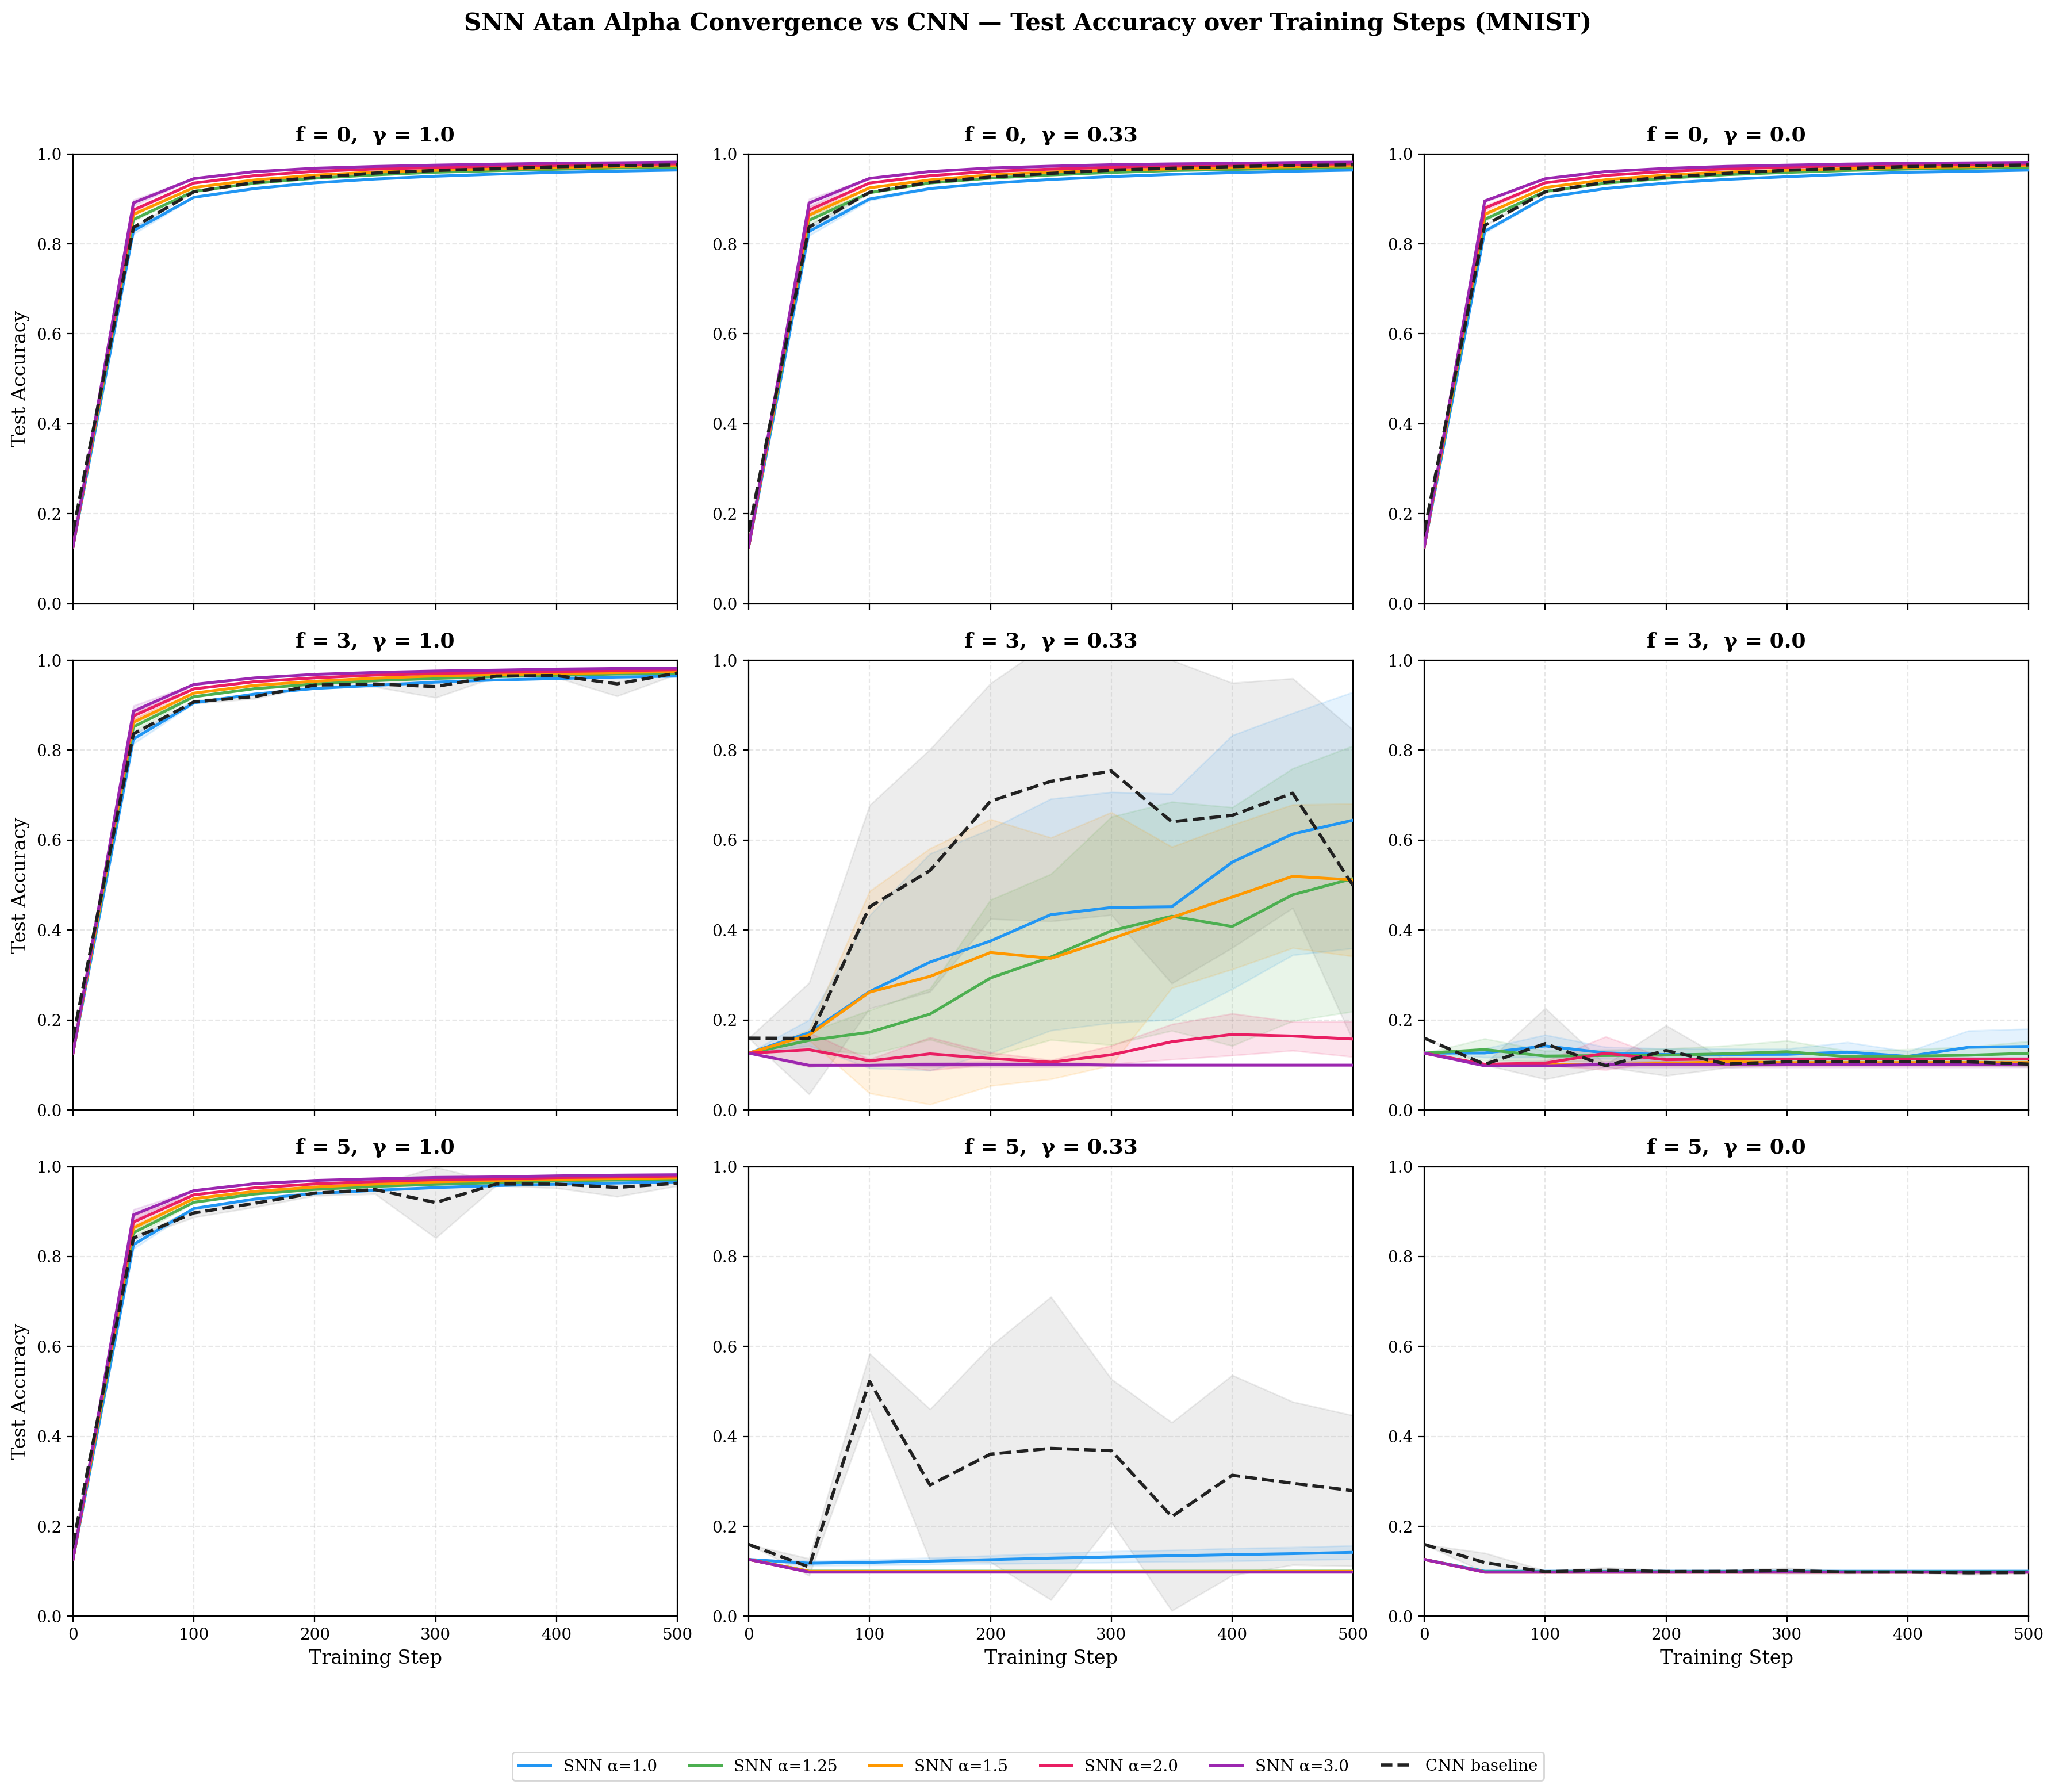
\includegraphics[width=0.9\textwidth]{test_accuracy_grid.png}
    \caption{Empirical Robustness Heatmaps comparing CNN and various SNN Surrogate Gradients. Note the vertical degradation of CNN vs the diagonal resilience of SNNs.}
    \label{fig:heatmaps}
\end{figure}

\section{The Variance Trade-off: Friction as a Defense}
The observed crossing point of robustness (CNN slightly better at IID, SNN vastly superior at Non-IID) can be explained by the inherent variance of the models.

\subsection{CNN: Zero Friction, Infinite Sensitivity}
In a perfectly IID setting ($\gamma = 1.0$), honest clients computing dense, continuous gradients in a CNN yield exactly identical updates. The spatial variance $\sigma^2$ is exactly zero. Robust aggregators (like Geometric Median) can perfectly isolate any Byzantine perturbation. Thus, CNNs tolerate a high $f$ at $\gamma=1.0$.
However, when $\gamma < 1.0$, the gradients diverge rapidly. The variance explodes towards infinity. The "honest cluster" expands drastically, allowing sophisticated attacks to hide within this massive variance. The robustness collapses vertically.

\subsection{SNN: The Baseline Noise and Bounding}
SNNs possess inherent "friction" due to discrete spiking, membrane integration, and surrogate gradient approximations. Therefore, even at $\gamma=1.0$, honest clients exhibit a baseline variance ($\sigma^2 > 0$). This explains why SNNs might tolerate slightly fewer attackers in perfectly ideal IID conditions.
Crucially, when data becomes heterogeneous ($\gamma < 1.0$), this same friction acts as a powerful shock absorber. The variance increases, but \textbf{slowly and linearly}, prevented from exploding by three intrinsic mechanisms.

\section{Intrinsic Defense Mechanisms of SNNs}

\subsection{Mechanism 1: The Bounding Effect of Surrogate Gradients}
Unlike ReLU activations in CNNs where gradients can scale infinitely with the error, SNN surrogate derivatives (ArcTangent, Triangular) possess a strict peak and decay to zero as the membrane potential deviates from the firing threshold.
This acts as a non-linear clipping mechanism. If extreme data heterogeneity or a Byzantine attack pushes the potential too far, the local gradient is naturally driven to zero. It is mathematically impossible to generate unbounded gradients, strictly limiting the amplitude of the variance and the strength of any injected perturbation.

\subsection{Mechanism 2: Temporal Integration as a Low-Pass Filter}
The Leaky Integrate-and-Fire (LIF) dynamics govern the membrane potential $U(t)$ over discrete timesteps $T$. In continuous time, this is represented by $\tau \frac{dU(t)}{dt} = -U(t) + R I(t)$, which is the canonical differential equation for a first-order \textbf{low-pass filter} with transfer function $H(s) = \frac{R}{1 + \tau s}$.
Attacks designed to bias the spatial update at a given iteration must sustain their perturbation across the temporal window to force a false spike. If the perturbation is not consistent, the "leaky" dynamic dissipates the malicious current before the threshold is reached.

\subsection{Mechanism 3: Sparsity and the ALIE High-Frequency Trap}
Advanced attacks like A Little Is Enough (ALIE) attempt to bypass defense mechanisms by applying a constant, low-frequency perturbation $\Delta W_{\text{ALIE}}$ to the model weights. In a dense CNN, this constant weight bias multiplies with a continuous input signal, generating a massive, low-frequency disruption that corrupts the output.

However, in an SNN, the input signal $S_{\text{in}}(t)$ is a \textbf{sparse spike train} (mostly zeros, rare ones). The input current perturbation is $\delta I(t) = \Delta W_{\text{ALIE}} \cdot S_{\text{in}}(t)$.
Because $S_{\text{in}}(t)$ is highly sparse, the constant weight perturbation is transformed into a \textbf{high-frequency, intermittent pulsatile signal}.
As established in Mechanism 2, the LIF membrane acts as a low-pass filter. High-frequency signals ($\omega \to \infty$ in Laplace domain) are heavily attenuated ($H(s) \to 0$). Therefore, the ALIE attack falls precisely into the SNN's trap: its constant spatial perturbation is converted into a sparse, high-frequency temporal noise that is smoothly absorbed and dissipated by the membrane leak before causing malicious spikes.

\section{Conclusion}
The SNN's robustness is not a simple scaling artifact, but a fundamental consequence of its non-linear spatio-temporal dynamics. Sparsity forces attacks into high frequencies, where the LIF low-pass filter neutralizes them, while surrogate gradient bounding prevents the spatial variance from exploding under data heterogeneity.

\end{document}
